\section{The Impact of False Detections on MOPS Performance \label{sec:appMOPS}}


We seek to develop an analytic understanding for the behavior of the MOPS results.
In particular, we want to be able to predict the numbers of tracklets and
candidate tracks for a given input number of true and false detections. In addition, we seek
to understand how these numbers scale with the search window width,
velocity cutoff when forming tracklets, the temporal separation of two
detections in a tracklet, and the density of false detections. For example, available
MOPS experiments indicate that the number of tracklets increases with
the square of the false detection density, but other scalings are unclear,
especially the behavior of false candidate tracks.

We first derive the simpler false tracklet rates, and then use these results to
discuss false candidate track rates. 


\subsection{Expected False Tracklet Rates \label{sec:tracklets} }

Given a detection in the first difference image, another difference image, obtained at a different epoch,
is searched for a matching detection to form a tracklet,  {\it e.g.} \citet{denneau13, kubica07}. For orientation,
the sky density of asteroids down to LSST $5\sigma$ faint flux limit ($r \sim 24.5$) is of the order
$\rho_{ast} \sim 100$ deg$^{-2}$. The predicted highest asteroid sky density for $r<24.5$,
on the Ecliptic, is up to about five times larger (with an uncertainty of about a factor of 2,
depending on model assumptions), and the density decreases rapidly with the ecliptic latitude.
A typical LSST observing night includes about 1000 visits, with two visits per night over
the active sky area. The nominal LSST field-of-view area is $A_{FOV}=9.6$ deg$^2$, with a
fill factor of 0.9, giving an effective field-of-view area of $A_{FOV}^{eff}=8.64$ deg$^2$. Hence,
the number of detected asteroids per night is of the order 500,000 (with implied two detections
per asteroid), although it can be significantly lower when the Ecliptic is not well covered (and
it could be a few times higher if the majority of visits were obtained along the Ecliptic).

The number of false detections due to (Gaussian) background fluctuations is
about $\rho_{bkgd} = 60$ deg$^{-2}$, assuming typical LSST seeing (0.8 arcsec)
and SNR$>$5. For a given seeing and SNR threshold, the rate of false detections can never be
lower than this estimate. This false detection rate decreases with the square of the seeing, and
strongly depends on SNR: the rate increases/decreases by as much as a factor of about ten
when SNR threshold is changed to 4.5 and 5.5, respectively (see \S\ref{sec:imDiff}).

Analysis of DECam images reduced using prototype LSST software, described in \S\ref{sec:imDiff},
shows a higher rate of detections in difference images, and a fraction of those detections
cannot be readily associated with true moving objects. This analysis implies a conservative
upper limit for the false detection rate of about $\rho_{FP} =  400$ deg$^{-2}$. This value
is conservative because analyzed DECam fields are close to the Ecliptic, with a significant but
not well known contribution from real asteroids (due to very faint flux levels, $r \sim 24$),
and it also includes true astrophysical transients that are not associated with static objects
(stars and galaxies). It is quite possible that the false detection rate might be several
times lower, though we will proceed with the most conservative estimate above.

The sky density of detections in difference images, $\rho_{det}$, is given by
the sum of contributions from true asteroids and false detections, $\rho_{det} = \rho_{ast} + \rho_{FP}
= 500$ deg$^{-2}$. When searching for a matching detection in another difference image, there are
two distinct types of behavior. Correct matches of detections of the same asteroid into tracklets follow the behavior
expected for correlated samples: as long as the object's angular displacement between the two epochs
is sufficiently larger than the seeing disk, while at the same time smaller than the search radius, the
number of matches (that is, the number of true tracklets produced per LSST pointing, assuming
two visits of the same area per night) is simply
\begin{equation}
                  N_{tracklet}^{true} = \rho_{ast}  \, A_{FOV}^{eff},
\end{equation}
With  $\rho_{ast} = 100$ deg$^{-2}$, $N_{tracklet}^{true} \sim 1,000$ per a pair of visits, and with
500 visit pairs per typical observing night, $N_{tracklet}^{true} \sim 500,000$ per night (same as
the number of detected asteroids in the active sky area, of course). Again,
this number can be much lower for fields far away from the Ecliptic, and a few times larger
for exceptionally good coverage of the Ecliptic. We emphasize that this number of true tracklets
does not directly depend on the search radius, nor the time elapsed between the two visits, as long
as they have their plausible values (about an arcminute, and a few tens of minutes, as discussed
further below).


\begin{figure}[t!]
\centering
\vskip -2.0in
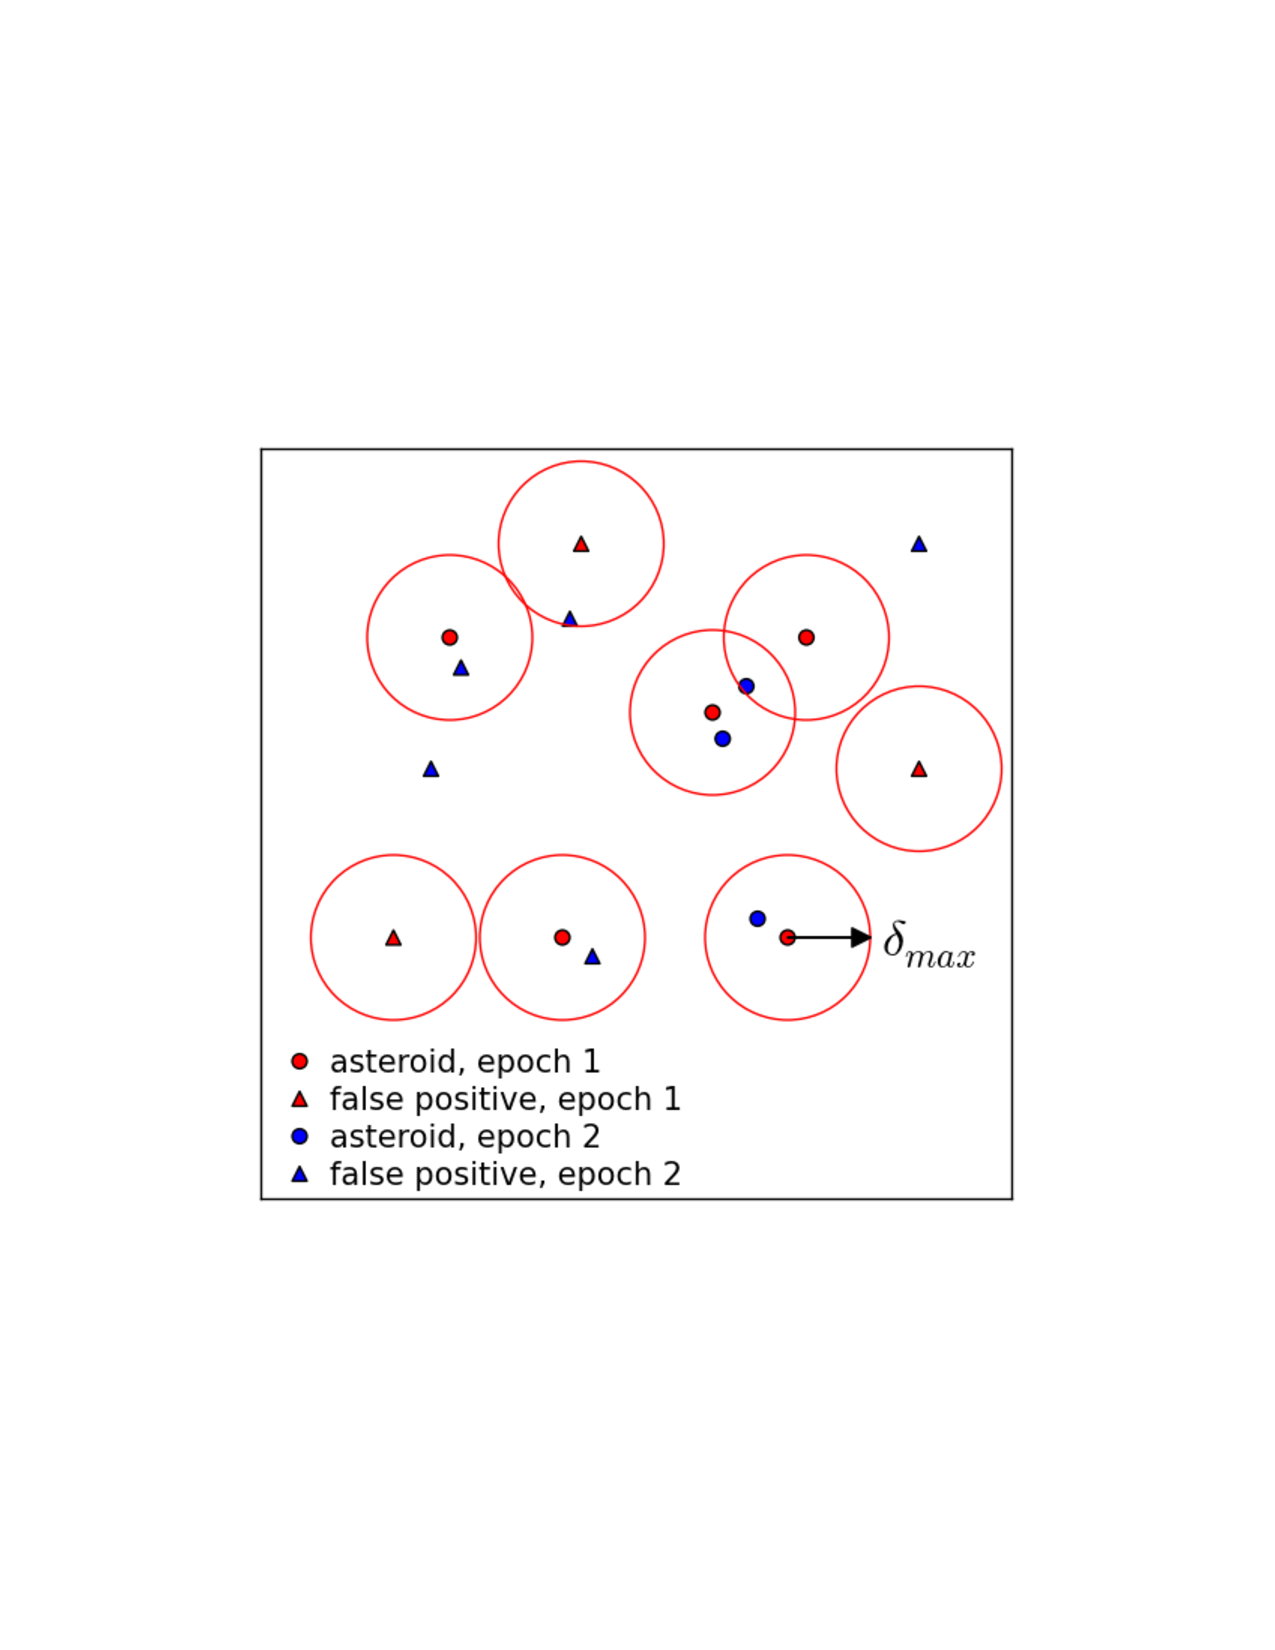
\includegraphics[width=0.95\textwidth]{figures/TrackSlide2}
\vskip -2.2in
\caption{An illustration of positional matching of detections to form tracklets.
Detections come in two flavors: asteroids (A, circles) and false detections (FP, triangles).
The figure shows the search for a matching detection in epoch 2 for each detection
in epoch 1, with a maximum search radius $\delta_{max}$. Note that there are six
possibilities: matches A-A, A-FP, FP-A, FP-FP, and orphaned A and FP.
\label{fig:TrackSlide2}}
\end{figure}

There are three other types of tracklets that follow the behavior for uncorrelated (random)
samples: associations of different asteroids, associations of asteroids and false detections,
and tracklets made of two false detections. Assuming the same $\rho_{det}$ in both
difference images, for each of $N_{det} = \rho_{det} \, A_{FOV}^{eff}$ detections in one image,
we search for a matching detection in another image (see Figure~\ref{fig:TrackSlide2}).
The search radius is given by
\begin{equation}
                     \delta_{max} = v_{max} \, \Delta t .
\end{equation}
Here $v_{max}$ is the  cutoff velocity and $\Delta t$
is the time elapsed between the two images. For LSST baseline cadence, $\Delta t$ is in
the range 20-60 minutes. The search area, $A_S = \pi \delta_{max}^2$, is then
\begin{equation}
\label{eq:AS}
      A_S = 0.0055 \left( v_{max}  \over {\rm deg \, day}^{-1} \right)^2 \, \left(\Delta t \over {\rm hour} \right)^2 {\rm deg}^2.
\end{equation}
To guide setting the cutoff velocity, simulations imply that 95\% of NEO detections have $v<1$ deg day$^{-1}$; with this threshold,
the completeness for main-belt asteroids is essentially 100\%. Objects moving faster than 1 deg day$^{-1}$ will
be easily resolved in LSST images and can be treated separately using specialized algorithms.
Adopting $v_{max} = 1$ deg day$^{-1}$,  and $\Delta t = 30$
minutes (which together  imply a search radius of $\delta_{max} = 1.3$ arcmin), gives a search area of
$A_S = 0.0014$ deg$^2$.


The expectation value for the number of matching detections within the search area $A_S$ (that is, the expected
number of tracklets per matching trial) is
\begin{equation}
                      p_{tracklet}^{false} =   \rho_{det}  \, A_S,
\end{equation}
and the total expected number of {\it false} tracklets for $N_{det}$ trials is thus
\begin{equation}
\label{eq:NttFalse}
           N_{tracklet}^{false} = N_{det} \, p_{tracklet}^{false} =  N_{visit} \, \rho_{det}^2 \, A_S \, A_{FOV}^{eff} = N_{visit} \, \rho^2_{FP}  \, A_S \, A_{FOV}^{eff} \,  \left(1 + 2 \eta + \eta^2\right),
\end{equation}
where $\eta = \rho_{ast}  / \rho_{FP} \sim 0.25$ (recall that $\rho_{det} = \rho_{ast} + \rho_{FP}$).
With $\rho_{ast} = 100$ deg$^{-2}$ and  $\rho_{FP} = 400$ deg$^{-2}$,
$N_{tracklet}^{false} \sim 3,000$ per pair of visits, and $N_{tracklet}^{false} \sim 1.5$ million per observing night with
$N_{visit}=500$ visit pairs. We note that the density of false tracklets ($\rho_{tracklet}^{false}=350$ deg$^{-2}$) is similar to
$\rho_{FP}$; this similarity is a consequence of choosing $\delta_{max}$ such that $\rho_{FP} A_S \sim 1$.

The first term in eq.~\ref{eq:NttFalse} is the largest and corresponds to tracklets made of two false
detections ($\sim1.0$ million), the second term corresponds to associations of asteroids and false detections,
and the third and the smallest term ($<0.1$ million) is due to incorrect associations of different asteroids.
For the chosen parameter values, the total number of tracklets is about 2 million per observing night, Given that
these choices are rather conservative, this estimate is essentially an upper limit; approximately,
{\it we expect of the order a million tracklets per observing night}.

To the first order ($\eta \approx 0$), the total number of tracklets per night is
\begin{equation}
    N_{tracklet} =  N_{tracklet}^{true} + N_{tracklet}^{false} =
       N_{visit} \, A_{FOV}^{eff} \, \left(\rho_{ast}  + \rho^2_{FP}  \, A_S \right).
\end{equation}
In addition to $N_{tracklet}^{false}$ scaling with the square of $\rho_{FP}$, as demonstrated using MOPS,
$N_{tracklet}^{false}$ scales with the square of
both $v_{max}$ and  $\Delta t$ (via the dependence on $A_S$). Therefore, if $\Delta t$ would be made
as small as 10 minutes by modifying the observing strategy, the resulting $N_{tracklet}^{false}$ would be about an
order of magnitude smaller (and $N_{tracklet}$ about three times smaller).  Hence, the shortening of $\Delta t$ is
a good mitigation strategy against high false detection rates in difference images\footnote{An
extreme example of this mitigation strategy would be to obtain two consecutive 30-second visits -- their
mid-exposure times would be separated by 34 seconds (additional 2 seconds due to shutter motion and another
2 seconds due to readout), which is sufficient to detect motion faster than about 0.1 deg day$^{-1}$.}.


\subsubsection{False tracklet velocity distribution \label{sec:falsev}}

False tracklets have randomly distributed velocities (motion vectors) with a cutoff given by $v_{max}$
(recall that $v_{max} = 1$ deg day$^{-1}$ was adopted above). The implied tracklet velocity is given by
\begin{equation}
                       v =  \delta / \Delta t,
\end{equation}
where $\delta$ is the angular separation of two detections. Since the number of tracklets
with separation $\delta$ increases linearly with $\delta$ (because the area of a circular
annulus is $2\pi r dr$), the false tracklet velocity distribution will increase linearly with
$v$ for $v<v_{max}$, and the vector orientation will be random. We show below that candidate
tracks can be efficiently pruned using this result.



\subsection{Expected False Track Rates \label{sec:tracks} }

In this section, we present an approximate estimate of the expected number of false candidate tracks.
Our goal is to derive the scaling of this number with the relevant input parameters, such as the true and false
tracklet rates per night ($N_{tracklet}^{true}=5\times10^5$ and $N_{tracklet}^{false}=1.5\times10^6$, respectively).
For a fiducial case, we assume that the search window is $N_w= 30$ days wide;  therefore, with $N_{tracklet} = 2\times10^6$
per night, there are $6\times10^7$ tracklets in the fiducial dataset. With about 4,300 deg$^2$ (500 pairs of visits)
of sky observed each night, the average density of (all) tracklets is $\rho_{tracklet} = 450$ deg$^{-2}$. Assuming
that on average the same field is revisited every $T_{revisit}=3$ days, the active area includes about 13,000 deg$^2$
of sky.

As discussed below in more detail, there are of the order 1000 different ways to chose a triplet of nights
from the search window. Given 10$^6$ tracklets per night, there are of the order
10$^{21}$ different combinations of tracklet triplets that could form a candidate track.
While this number of candidate tracks is obviously prohibitively large to test for consistency
with heliocentric Keplerian motion, it can be sufficiently reduced (to about the same number
as the number of true tracks along the Ecliptic) using pre-filtering steps based on tracklet motion
vectors, summarized below and following similar methods as described in \citet{denneau13, kubica07}. 

In the first step, the motion vector of a tracklet from the first night is linearly extrapolated
to the second night and tracklets from the second night are searched for within a radius set
by the orbital curvature (which dominates over LSST's expected astrometric errors). With appropriate use of
kd-trees and similar algorithms for fast searches, only a small fraction (of the order a percent)
of tracklets from the second night need to be examined in detail. The cutoff radius varies
from $\sim$1 arcmin for the case of two consecutive nights to $\sim$1 deg. for a 15-day separation
(as discussed in detail further below). In addition, the velocity of second tracklet is required
to be consistent with the velocity implied by the positions of the two tracklets. After
this step, there are about 10$^{10}$ tracklet pairs for further processing (for $N_w=30$
days).

In the second step, parameters of a parabola (for each coordinate) are constrained using the
positions and velocities of the two tracklets, and this parabolic motion is extended to a third
night to search for matching third tracklet. This step results in up to 10$^{11}$ candidate
tracks.

Using the positions of the three tracklets, parabolic motion (for each coordinate) is fit
in the third step. The velocities implied by this motion are compared to the velocities for
the first and third tracklet. This filtering step reduces the number of candidate tracks
by a factor of about 10$^{5}$ and brings the number of false candidate tracks to
the same range as the number of true tracks close to the Ecliptic. These three matching
and pre-filtering steps bring the number of candidate tracks to a level that
can be easily handled by the IOD filtering step.

We now proceed with a more detailed description of three pre-filtering steps
for candidate tracks.

\subsubsection{The Number of 3-night Combinations in the Search Window}

We can form a candidate triplet of tracklets by first choosing the middle (second) tracklet.
For simplicity, we will measure time of observation in integer days. Given $N_w$ nights
in the search window, the middle tracklet comes from night indexed $k$, with
$2 \le k \le (N_w-1)$. The night that contributes the first tracklet is indexed by $j$,
with $1 \le j \le (k-1)$, and the night that contributes the third tracklet is indexed by $l$,
with $(k+1) \le l \le N_w$. The number of 3-night combinations can be expressed in a closed
form
\begin{equation}
\label{eq:N3}
  N_{3nights} = \sum_{k=2}^{N_w-1} \, (k-1)\, (N_w-k) =\frac{1}{6}N_w^3 - \frac{1}{2}N_w^2 + \frac{1}{3}N_w,
\end{equation}
giving $N_{3nights} = 455$ for $N_w=15$ and $N_{3nights} = 4,060$ for $N_w=30$.  Note
that for large $N_w$, $N_{3night}$ is proportional to $N_w^3$ -- the number of 3-nights
combinations increases by about an order of magnitude when $N_w$ is doubled from
15 days to 30 days.

It is important to point out that in steady-state processing a single night is added to the
window from the previous night, and the first night is dropped. Therefore, only the {\it new}
3-night combinations, where the third night is the last night in the search window, need
be considered in steady-state processing (and the ramp up is easy because of the gradually
increasing search window size). It is straightforward to show that the number of such
3-night combinations is
\begin{equation}
\label{eq:N3n}
  N_{3nights}^{new} = \sum_{k=2}^{N_w-1} \, (k-1) =\frac{1}{2}N_w^2 - \frac{3}{2}N_w + 1,
\end{equation}
yielding $N_{3nights}^{new} = 91$ for $N_w=15$ and $N_{3nights}^{new} = 406$ for $N_w=30$.
Note that $N_{3nights}^{new} \sim N_{3nights} / 10)$ for $N_w=30$, which represents
a significant reduction.


\subsubsection{The Tracklet Motion Vector Accuracy \label{sec:astromerrors}}

In addition to its mean position at the mean epoch, each tracklet constrains the motion vector.
Typical astrometric errors for LSST detections will range from about 50 mas at SNR=100 (dominated
by systematics) to 150 mas at SNR=5 (dominated by random errors). For simplicity, we will assume 
hereafter that the astrometric errors are
$\sigma_a=150$ mas for all detections, or $\sim 100$ mas per coordinate. With a temporal
separation of two detections in a tracklet of $\Delta t$, the motion vector is measured with an
accuracy per coordinate of
\begin{equation}
\label{eq:sigv}
          \sigma_v = 3.6 \, \left({\rm hour} \over \Delta t\right) \,\,\, {\rm arcsec} \, {\rm day}^{-1}.
\end{equation}
With a typical $\Delta t = 30$ min, and assuming a linear motion in each ecliptic coordinate (longitude
$\lambda$ and latitude $\beta$), each coordinate can be predicted at time $t$ with an accuracy of
\begin{equation}
            \sigma_x = 7.2 \, \Delta k \,\,\, {\rm arcsec},
\end{equation}
where $\Delta k$, in days, is the elapsed time between the mean tracklet epoch and time $t$
(for example, the number of nights between the first and the second tracklet in a candidate track).
For illustration, when $\Delta k = 7$ days, $\sigma_x = 50$ arcsec, which is roughly the same
as the typical detection separation in a tracklet, and comparable to typical distance between
two tracklets.  However, it turns out that the positional discrepancies due to a simple linear extrapolation of
motion for NEOs are an order of magnitude larger than the astrometric measurement errors
even in case of two consecutive nights ($\sim$1 arcmin vs. 7 arcsec, respectively). We proceed with
a quantitative analysis of the required matching radius using simulated orbits for main-belt asteroids
and NEOs.



\subsubsection{Initial Linking of Tracklets into Candidate Tracks}

Given a combination of 3 different nights from the search window, for each tracklet
from the first night we can linearly extrapolate its motion vector and require that the
measured  position of a tracklet from the second night is consistent with the predicted
position (the night ordering can be reversed from 1-2-3 to 3-2-1). Given a tracklet from
the first night, it is not necessary to search through all tracklets from the second night.
Search methods such as kd-trees can be used to rapidly reject tracklets that have no
chance of being matched. As an example of a ``poor man's'' rapid search, consider the
fact that tracklets from each night are already ``self-organized'' into about 500 visits,
which correspond to a field of view with a diameter of 3.5 deg. It is easy to show that with
an upper limit on possible motion of 5 deg, only 19 visits from the second night need to be
searched for matching tracklets. This significant reduction of a factor of $\sim$25 in
the number of candidate matching tracklets can be further boosted by applying more
sophisticated tree algorithms.

Using ecliptic longitude $\lambda$ for illustrative purposes, the predicted search position for the
second tracklet is
\begin{equation}
\label{eq:lambdaPred}
               \lambda_2^\ast = \lambda_1 + v_1^\lambda \, \Delta T_{21},
\end{equation}
where $\Delta T_{21}$ is the elapsed time between the epochs of the first and second tracklet,
and $v_1^\lambda$ is the longitudinal component of $v_1$, the motion vector for the first
tracklet, {\it divided by} cos($\beta$). The expectation value for the number of matches in
an ellipse (see the left panel in Figure~\ref{fig:TrackSlide1})
centered on predicted position ($\lambda_2^\ast, \beta_2^\ast$), and within limits $r_\lambda^{max}$
and  $r_\beta^{max}$ along the Ecliptic longitude and latitude, is given by
\begin{equation}
\label{eq:Nmdk}
     N_{match}(\Delta k) = \pi \, r_\lambda^{max} \, r_\beta^{max}  \, \rho_{tracklet} \left({1 \, {\rm day} \over T_{revisit}}\right)
\end{equation}
where the division by $T_{revisit}$ reflects the fact that each field is revisited on average only
every $T_{revisit}$ days (statistically speaking; the number of matches is zero for all but one
night out of $T_{revisit}$ nights).

The extrapolation given by eq.~\ref{eq:lambdaPred} implies that orbits can be approximated by
linear motion (in each coordinate) over time $\Delta T$. This is an incorrect assumption
due to orbital curvature and we analyze this effect using orbital simulations of MBA and NEO
samples described in \S\ref{sec:MAFdetails}.

Analysis of simulated samples shows that an adequate acceleration limit\footnote{See also
Figure 16 in \citet{LDM-156}.} is $a^{max}=0.02$ deg day$^{-2}$: essentially
all main-belt asteroids and more than 95\% of NEOs satisfy this criterion. If this acceleration
were constant during an interval of $\Delta k$ days, the maximum positional discrepancy
would be proportional to $\Delta k^2$. Numerical analysis of the simulated orbital motions
suggests that an approximately constant selection completeness (as a function of $\Delta k$)
is attained for
\begin{equation}
\label{eq:matching1}
                r_\beta^{max} = A \, \Delta k^{1.5}.
\end{equation}
with $A=1.0$ arcmin, and $r_\lambda^{max} = 5 \, r_\beta^{max}$. The achieved completeness for
a fiducial $\Delta k$=7 days is 0.99 for MBAs and 0.95 for NEOs, with very little dependence
on $\Delta k$ for 1 day $\le \Delta k \le$ 21 days (per single search window -- note that most
objects will have multiple discovery chances).  With this linear motion model, the number
of matched tracklets per single trial tracklet is
\begin{equation}
\label{eq:Nmdk2}
   N^{L}_{match}(\Delta k) = 1.96 \, \left({1 \, {\rm day} \over T_{revisit}}\right) \,
                    \left( \rho_{tracklet}  \over 450 \, {\rm deg}^{-2} \right) \, (\Delta k)^3.
\end{equation}
For example,  the expected number of matches for $\Delta k$=7 days is $\sim$224
(a 19 arcmin by 93 arcmin matching ellipse), and rises to $\sim$6,000 for
$\Delta k$=21 days.

Given the two matched tracklets, we can then approximate the motion as a parabola
\begin{equation}
\label{eq:parabola}
          \lambda(t) = \frac{1}{2}a^\lambda \, t^2 + v^\lambda \, t + \lambda_1,
\end{equation}
where $t = mjd - mjd_1$ (and analogously for latitude $\beta$).  Using the tracklet
positions and the motion vector of the first tracklet, the acceleration can be directly
estimated as
\begin{equation}
 \label{eq:accPred}
             a^\lambda = 2 \, {\lambda_2- \lambda_1 - v_1^\lambda \Delta T_{21} \over \Delta T^2_{21}},
\end{equation}
and the predicted velocity for the second tracklet can be estimated from
\begin{equation}
\label{eq:v2cut}
        (v^\lambda_2)^\ast =  a^\lambda \,\Delta T_{21}  + v_1^\lambda =
      {2(\lambda_2- \lambda_1) \over \Delta T_{21}}  - v_1^\lambda.
\end{equation}

We find that a comparison of $v_2^\lambda$ and $(v^\lambda_2)^\ast$ can further decrease
the number of false tracks (recall \S\ref{sec:falsev}); with tolerances of $\Delta v^\lambda < 0.3$ deg/day and
$\Delta v^\beta < 0.07$ deg/day (applied simultaneously for both coordinates as an
elliptical condition), the reduction is about a factor of 50 (for $v_{max}$ = 1 deg day$^{-1}$),
with only a minimal impact on the sample completeness. Therefore, depending on $\Delta k$, the number of tracklet
pairs per trial tracklet  to continue processing ranges from $\sim$4 for $\Delta k$=7 days to
$\sim$120 for $\Delta k$=21 days. When added over all possible pairs of nights (with
$T_{revisit}=3$ days), the total number of candidate tracklet pairs normalized by
the number of tracklets per night ranges from 350 for $N_w=15$ days to 13,400 for $N_w=30$ days.
Therefore, the following, more involved, selection steps need to be executed for
no more than about $10^{10}$ tracklet pairs (for $N_w=30$ days; and only for $3\times10^{8}$
pairs when $N_w=15$ days). These numbers are significantly lower than the naive estimate of
10$^{15}$ ($10^3\times10^6\times10^6$).

We note that in steady-state processing, the new candidate tracklet pairs need to
be evaluated only for pairs of nights where the second night is the penultimate
night in the search window (all other combinations will have been already computed
on previous days). Because the caching of results from previous night is not
yet implemented in MOPS, we don't account for this reduction (of about a factor of
3 to 6) in the analysis presented here.

Given the acceleration estimate from eq.~\ref{eq:accPred}, the position of the third
tracklet can be predicted from
\begin{equation}
\label{eq:lambdaPred3}
  \lambda_3^\ast = \frac{1}{2} a^\lambda \, \Delta T_{32}^2 + v_2^\lambda \, \Delta T_{32} + \lambda_2.
\end{equation}
Similarly to eq~\ref{eq:matching1}, an approximately constant selection completeness
can be achieved using
\begin{equation}
\label{eq:matching2}
                r_\beta^{max} = B \, \Delta k^{1.5}.
\end{equation}
with $B=0.2$ arcmin, and $r_\lambda^{max} = 5 \, r_\beta^{max}$. Note that the search
area is now 25 times smaller than in the first case, thanks to parabolic rather
than linear extrapolation. Therefore, the number of matched tracklets per single
trial tracklet pair is
\begin{equation}
\label{eq:Nmdk3}
     N^P_{match}(\Delta k) = 0.078 \, \left({1 \, {\rm day} \over T_{revisit}}\right) \,
                    \left( \rho_{tracklet}  \over 450 \, {\rm deg}^{-2} \right) \, (\Delta k)^3,
\end{equation}
and the expected number of matches ranges from 9 for $\Delta k$=7 days to
$\sim$240 for $\Delta k$=21 days.

%####
The total number of candidate tracks per single trial tracklet, for all possible 3-night
combinations (where the third night is the last night in the search window) is
\begin{equation}
\label{eq:Ntt}
   N_{tracklet}^{tracks} = 3.2\times10^{-3} \, \left( \rho_{tracklet}  \over 450 \, {\rm deg}^{-2} \right)^2 \, \left({1 \,{\rm day}\over T_{revisit}}\right)^2 \, \sum_{k=2}^{N_w-1} \sum_{j=1}^{k-1} \, (k-j)^3 \, (N_w-k)^3.
\end{equation}
The normalization constant is equal to $1.96\times0.078\times(\Delta v^\lambda
\Delta v^\beta/v_{max}^2)$, where the term in parenthesis is $\sim0.02$. This
normalization gives the number of candidate tracks per search window normalized
by the number of tracklets per night (which is assumed constant for all nights).
The two terms in the sum reflect the multiplication of the number of matches found
in the first selection step (linear extrapolation from the first to the second night,
eq.~\ref{eq:Nmdk2}) and the number of matches found in the third selection step
(parabolic extrapolation from the second to the third night, eq.~\ref{eq:Nmdk3}).

The sums in eq.~\ref{eq:Ntt} can be evaluated analytically, but the result is cumbersome.
Using numerical evaluation (with $T_{revisit}=3$ days), we find that the number of candidate
tracks per tracklet ranges from $\sim600$ for $N_w=15$ days to $\sim174,000$ for
$N_w=30$ days ($N_{tracklet}^{tracks}$ scales with $N_w^8$ when the third night must be
the last night from the search window).
Therefore, the matching of the candidate third tracklet brings the number of candidate
tracks per search window to the range 10$^{9}$ - 10$^{11}$. The ratio of false candidate tracks
to true tracks is in the range 10$^{3}$ - 10$^{5}$, depending on $N_w$. Despite the reduction by
a factor of  about $10^{10}$ to $10^{12}$ from the combinatorial number of tracklet triplets,
another significant reduction is required before the IOD step can be attempted.


\begin{figure}[th!]
\centering
\vskip -2.6in
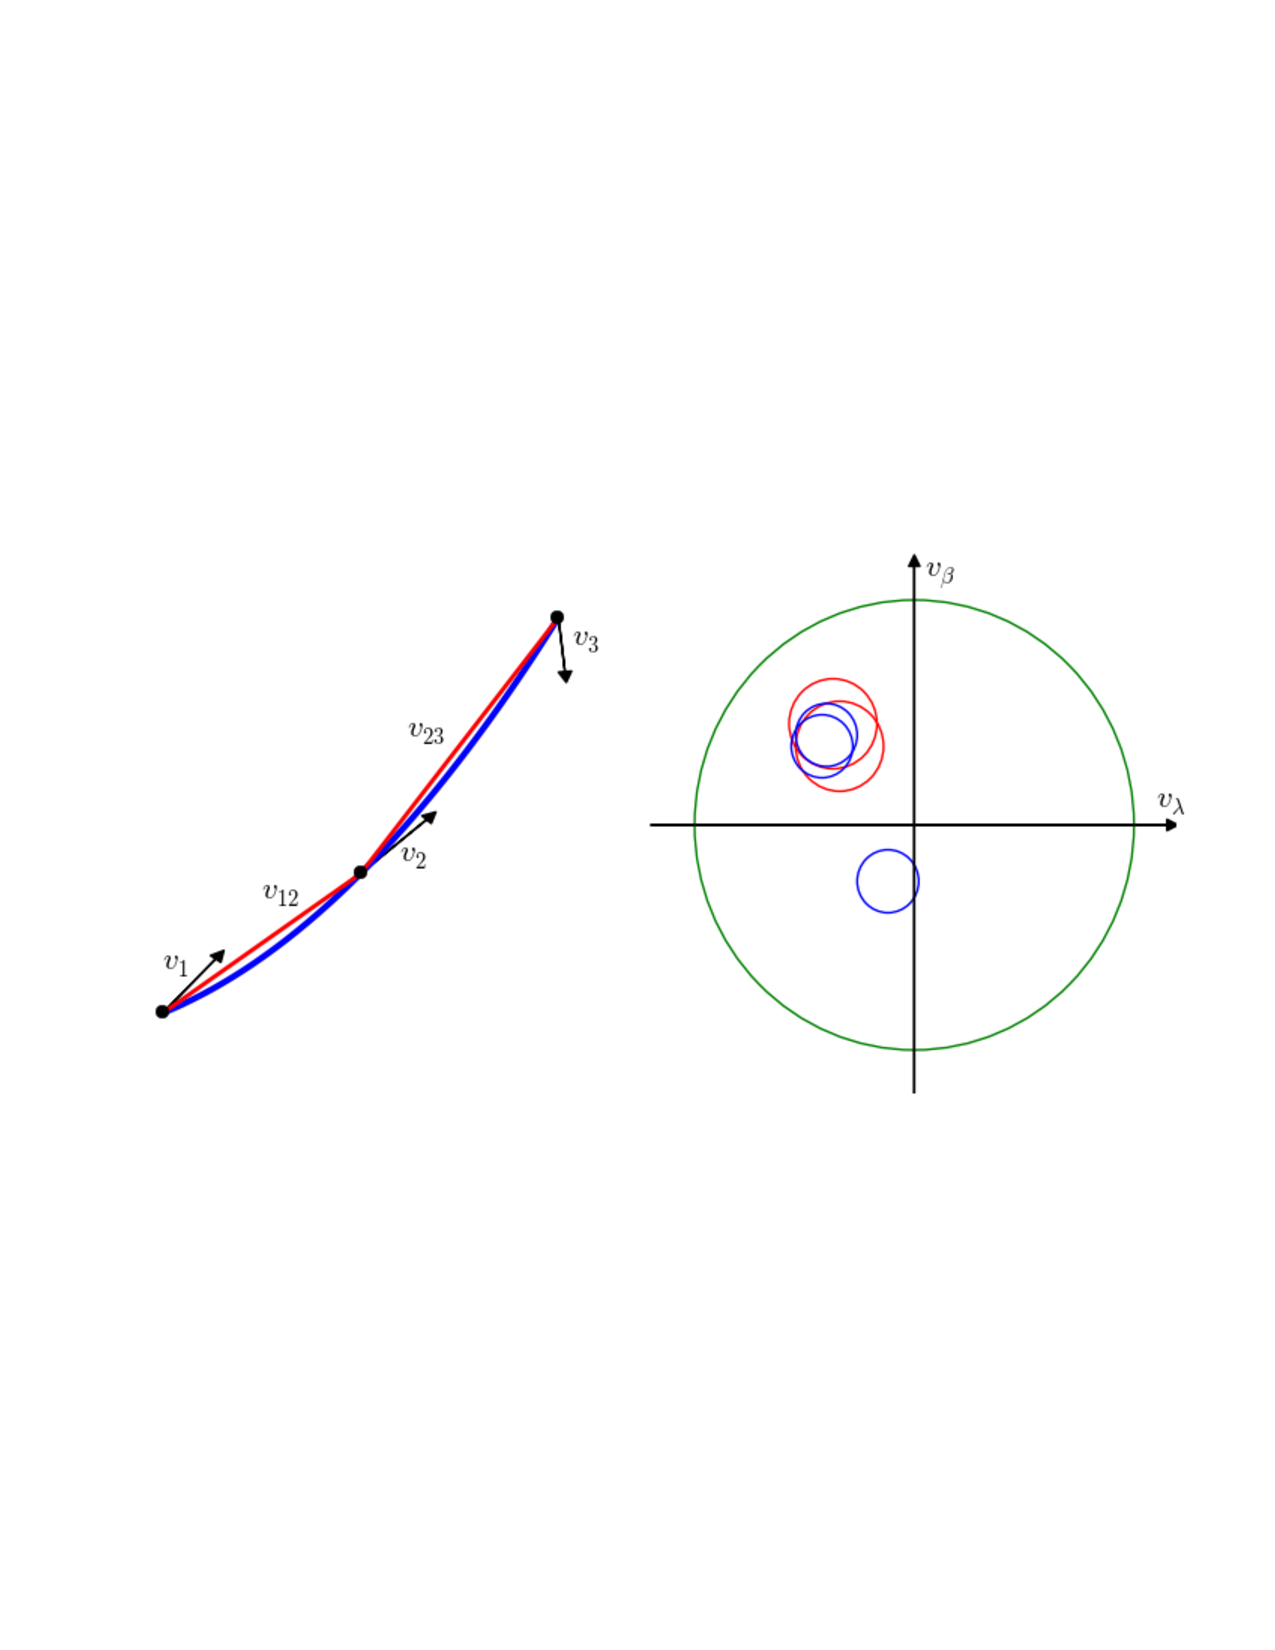
\includegraphics[width=0.95\textwidth]{figures/TrackSlide1}
\vskip -2.7in
\caption{The left panel shows a hypothetical asteroid trajectory as the curved blue line (with
the curvature greatly exaggerated). Three tracklets are shown by the black dots; the
two individual detections per tracklet are not shown, but are implied by the three measured
motion vectors ($v_1$, $v_2$ and $v_3$). The third tracklet illustrates a false tracklet.
The motion vector of the first tracklet is linearly extrapolated to the time of the second
tracklet and matched within the red ellipse. The first two tracklets are then used to
constrain parabolic extrapolation, shown by the green dotted line, which is then matched
within the green ellipse. Given three candidate tracklets, a parabola is fit to their positions
and predicted motion vectors are computed for each tracklet (the blue vectors in the middle
panel). This comparison is illustrated in the right panel, where the circle signifies the cutoff
velocity for forming tracklets. Note that the third tracklet has a measured velocity ($v_3$)
that is inconsistent with the predicted velocity ($v_3^\ast$). The consistency radii are discussed
in the text.
\label{fig:TrackSlide1}}
\end{figure}

%%%%   add references to the figure (left panel)  in above sections

\subsubsection{Using Tracklet Motion Vectors to Prune Candidate Tracks}

The positional matching described above didn't use strong constraints on the tracklet velocities
for the first and third tracklets. Since false tracklets (anything other than a true 
asteroid-asteroid pair of detections) have random velocities, 
velocity filtering can further reduce the number of false tracks.
With three candidate tracklets, a parabolic motion (see eq.~\ref{eq:parabola}) can be fit {\it without}
using tracklet velocities. This fit predicts the velocity of each tracklet from the first derivative of
the fit, which can then be compared to each measured velocity. Figure~\ref{fig:TrackSlide1}
illustrates a situation where, e.g., $v_3$ is inconsistent with the velocity predicted using such
parabolic fit.

The consistency tolerances are driven by the orbital curvature and acceleration, rather than
by the velocity measurement errors (velocities are measured with a precision of about 0.001
deg day$^{-1}$, see eq.~\ref{eq:sigv}). Analysis of the simulated samples described in
\S\ref{sec:MAFdetails} shows that velocity tolerances of $\delta v_\lambda^{max}$=0.12 deg day$^{-1}$
for the longitudinal component and $\delta v_\beta^{max}$=0.03 deg day$^{-1}$ for the latitudinal component
reject most false tracklets with only a few percent effect (per single discovery attempt) on overall
sample completeness.

The probability that a random false tracklet velocity will be consistent with a given expected
velocity is approximately (assuming a uniform distribution of false tracklet velocities)
\begin{equation}
        p_v =  { \delta v_\beta^{max} \, \delta v_\lambda^{max} \over  v_{max}^2 }
\end{equation}
With $v_{max} = 1$ deg day$^{-1}$, $p_v = 0.0036$. In reality, this probability is a bit smaller because
the false tracklet velocity distribution is not uniform (it is biased towards the velocity cutoff).
Finally, the probability that all three tracklets have velocities consistent with those
implied by their positions is $p_v^2 \sim 10^{-5}$ (not $p_v^3$ because $v_2$ was already
subjected to a fairly stringent cut, see eq.~\ref{eq:v2cut}; a more stringent cut here
would provide a reduction by about a factor of five, which we ignore)

This significant reduction in the number of candidate false tracks, due to filtering velocities
of the first and third tracklets, brings it to the range 10$^{4}$ - 10$^{6}$, which is smaller or at
most about the same as the number of true candidate tracks (on the Ecliptic). 

False tracks can also arise from incorrect matches of true (asteroid-asteroid) tracklets 
from different asteroids and these do not have a random distribution
of velocities. We discuss the impact of this below, when evaluating the results 
of numerical (instead of analytical) scaling evaluations, however the increase in
number of false tracks is small, as the density of false detections is much larger than
the density of asteroids.

With this final
reduction, the IOD step can be attempted with no more than about 10$^6$ candidate tracks per
search window.



\subsubsection{The scaling of the number of false tracks with the density of false detections}

The final number of false tracks can be computed using eq.~\ref{eq:Ntt}, after multiplying
the normalization constant by $p_v^2$ to account for velocity filtering. Numerical evaluation
shows that the expected number of false tracks per tracklet can be described as
\begin{equation}
\label{eq:NttFinalFit}
   N_{tracklet}^{tracks} = 2.4 \, \left({N_w\over 30\, {\rm day}}\right)^8 \, \left( \rho_{tracklet}  \over 450
        \, {\rm deg}^{-2} \right)^2 \, \left( {3\,{\rm day} \over T_{revisit}} \right)^2 \,
         \left( {1 \, {\rm deg} \, {\rm day}^{-1}  \over  v_{max} }\right)^6.
\end{equation}
Note the very steep dependence on $N_w$: the large power-law index (8) is a result of the two
powers of 3 under sum in eq.~\ref{eq:Ntt}, and the scaling of the number of three-night
combinations with $N_w^2$ from eq.~\ref{eq:N3n}. The scaling of $N^{falsetracks} = N_{tracklet}^{tracks} \, N_{tracklet}$
with the density of false positive detections is very steep, too. Since $N_{tracklet}$ and $\rho_{tracklet}$
are approximately proportional (in the limit $\rho_{ast}=0$) to $\rho_{FP}^2$ (see eq.~\ref{eq:NttFalse}),
the number of false candidate tracks approximately scales with $\rho_{FP}^6$. 
$N_{tracklet}^{tracks}$ scales with $v_{max}^{-6}$ because of velocity filtering for three tracklets,
with each of the three steps giving a $v_{max}^{-2}$ contribution). 
Since $N^{falsetracks}$ scales with $\rho_{tracklet}^3$, and $\rho_{tracklet}$ scales with $v_{max}^2$
(due to dependence of $A_S$ on $v_{max}$, see eq.~\ref{eq:AS}), $N^{falsetracks}$ is approximately 
independent of $v_{max}$ (but note that the number of intermediate filtering operations does 
depend on $v_{max}$). 

Without the limiting $\rho_{ast}=0$  approximation, eq.~\ref{eq:NttFalse} implies a shallower scaling
of the number of false candidate tracks, $N^{falsetracks}$ with $\rho_{FP}$.
We have determined numerically that the scaling of the number
of false candidate tracks per search window with the density of false detections in difference
images, as well as other relevant parameters, is well described by
\begin{equation}
\label{eq:falsetracks}
   N^{falsetracks} = 4.5 \times 10^6 \, \left( {N_w \over 30 \, {\rm day} } \right)^{8} \left( {\rho_{FP} \over 400 \, {\rm deg}^{-2} }\right)^{3.7}
    \left( {\Delta t  \over 30 \, {\rm min}} \right)^{2.7}
     \left( { 1 \, {\rm deg} \, {\rm day}^{-1} \over v_{max} }  \right)^{1.3}.
\end{equation}
This numerical approximation is only valid around above {\it fiducial values} of various 
parameters\footnote{For example, eq.~\ref{eq:falsetracks} cannot be used to conclude that
an infinitely large $v_{max}$ cutoff would result in no false tracks.}, 
and assumes $\rho_{ast}=100$ deg$^{-2}$ and $T_{revisit}=3$ days. With fiducial parameters, and 
when $\rho_{ast}=0$, the number of false tracklets per night is $\sim10^6$, and the number of false 
tracks per search window with $N_w=30$ days is about 550,000. For $N_w=15$ days,  the number 
of false tracks drops to $\sim2,000$. 

We note that the relevant quantity that determines the number of false candidate tracks is {\it not}
the ratio of false to real (asteroid) detections in difference images, but rather the overall number 
(and density) of false detections.

The scaling result given by eq.~\ref{eq:falsetracks} may prove useful when optimizing cadence
and search strategy, as well as for sizing the required computational resources. For example,
for the rate of 8,200 deg$^{-2}$ false detections from Pan-STARRS1, one would expect a factor
of $7\times10^4$ more false candidate tracks that discussed above (that is, about $10^{11}$).
Even with $N_w$=15 days, the predicted number of false candidate tracks remains of the
order 10$^9$.

Although MOPS algorithms operate in a different way, these analytic probabilistic considerations
explain why the number of candidate tracks produced in MOPS experiments stays approximately
the same (to within a factor of two) even when the number of input tracklets per night is increased
by about an order of magnitude. With $N_{tracklet}^{tracks} \sim2$, the number of  candidate
tracks (both true and false) per search window is about $N^{tracks} \sim 5\times10^6$ for $N_w= 30$ days,
that is, not overwhelmingly larger than the number of true tracks (500,000). In other words, the ratio of
false to true detections of 4:1 generates a ratio of false to true tracklets of 3:1 and a ratio of false to true
candidate tracks of 10:1 (for $N_w=15$ days and $\rho_{ast}=100$ deg$^{-2}$, the ratio of false to true
candidate tracks drops to below 5\%).

This similarity in the number of true and false candidate tracks is in good
agreement with the results of MOPS simulations\footnote{See the top left panel
in Figure 21 in \citet{LDM-156}} (though note that those simulations used more aggressive filtering
based on ``parabolic motion plus topocentric correction'' model, and thus obtained a factor of a few
lower counts of candidate tracks).
